% !TEX root = ../report.tex

\clearpage
\chapter{Pattern Documentation}
\label{ch:patterns}


\section{Core}
\subsection{Layers}
% see https://www.docker.com/sites/default/files/what-is-vm-diagram.png

\begin{figure}[H]
\centering
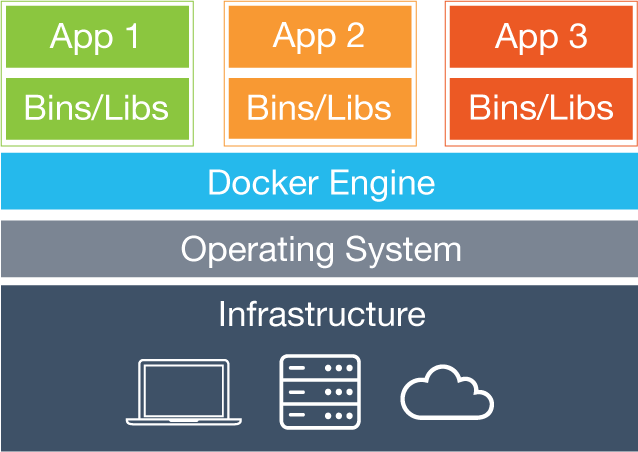
\includegraphics[scale=0.4]{5-patterns/images/what-is-vm-diagram.png}
\caption{A layered overview of the Docker. Source \cite{whatisdocker}}
\label{fig:layers-pattern}
\end{figure}

\begin{description}
\item [Traceability]~\\
The Layers pattern can be deducted from the online documentation\cite{dockerarchi}.

\item [Source]~\\
Architectural patterns revisited -- a pattern language, P. 29 \cite{avgeriou2005architectural}

\item [Issue]~\\
For a good encapsulation, each instance of docker is modeled using layers that interact with each other.

\item [Assumptions/Constraints]~\\
The interaction or communication between layers is carried out through socket, RESTful, or TCP/IP connection.

\item [Solution]~\\
Docker utilizes layers pattern. The system is modeled using layers and each component resides on a specific layer. An example can be seen in Figure \ref{fig:layers-pattern}.

\item [Rationale] ~\\
By separating each component in separated layers, the system will be more modular and have better security.

\item [Implications]~\\
There must be a clear closure of each layer. Communications protocol must also be defined.

\item [Related Patterns]~\\
\begin{itemize}
	\item Client-server
\end{itemize}
\end{description}

\clearpage
\subsection{Client-Server}
% see https://docs.docker.com/engine/introduction/understanding-docker/
% also nice image we can borrow: https://docs.docker.com/engine/article-img/architecture.svg
\begin{figure}[H]
\caption{An overview of the Docker architecture, showing the client and daemon. Source: \cite{dockerarchi}.}
\centering
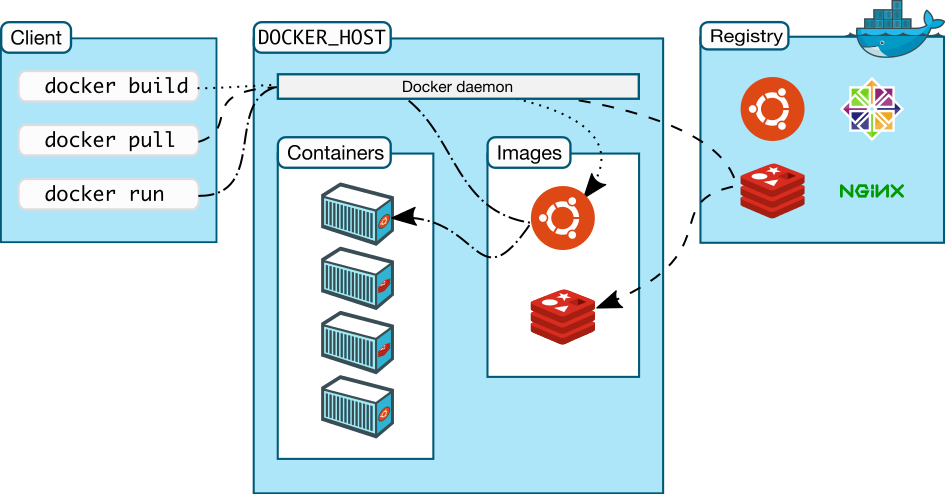
\includegraphics[scale=0.4]{4-softwarearch/images/architecture.png}
\end{figure}

\begin{description}
\item [Traceability]~\\
The Client-Server pattern can be deducted from the online documentation\cite{dockerarchi}.

\item [Source]~\\
Architectural patterns revisited -- a pattern language, P. 29 \cite{avgeriou2005architectural}

\item [Issue]~\\
For good interoperability, it should be possible for Docker containers to be started remotely. A single interface should be able to control containers on numerous hosts.

\item [Assumptions/Constraints]~


\item [Solution]~\\
Docker uses a Client-Server architecture. The client, a binary supplying a command-line interface, act as the primary interface for the user. The user enters commands into this client, which are then send to a server: the docker daemon. 

\item [Rationale] ~\\
The daemon is a background process, which supplies the requested services to the client. The daemon exposes a REST interface.

For Docker, the client can be configured to connect to other daemon processes than the one running on the local machine. It can be configured to connect to remote Docker daemons as well, allowing the user to issue commands to daemons running remotely.

\item [Implications]~\\
The use of the Client-Server pattern results in two different executable binaries: a daemon and a client. 

The use of a separated client handling the user interaction increases the modularity.
Furthermore, it increases the interoperability, since the client can send commands to daemons running on remote machines and the local machine.

All the services offered by the daemon have to be made available to the client using a REST interface.


\item [Related Patterns]~\\


\end{description}

\subsection{Shared repository}
\textit{Can we consider the docker registry a shared repository?}

\subsection{Plugin}
%TODO image
\begin{description}

\item [Traceability]~\\
The existence of Docker Plugins becomes apparent from it's documentation at \cite{dockerplugindocs}.

Additionally, the directories \verb|docker/pkg/plugins/| \footnote{\url{https://github.com/docker/docker/tree/master/pkg/plugins}} and \verb|  docker/daemon/graphdriver/plugin.go| \footnote{\url{https://github.com/docker/docker/blob/master/daemon/graphdriver/plugin.go}} (among others) in the project's repository contain the code for discovering plugins and the interfaces the plugins should implement.

\item [Source]~\\
Patterns of Enterprise Application Architecture, P. 499 \cite{eaa}

\item [Issue]~\\
The users of Docker want to have customization, by extending Docker with third party custom-built tools. This customization means that third parties should be able to write plugins that extend Docker's core functionality.\cite{dockerpluginblog}

The implementation of such plugins is only available at runtime.

\item [Assumptions/Constraints]~

\item [Solution]~\\
Docker uses the Plugin pattern to link the implementation of the interfaces of several extendable components with third-party implementation at runtime.

\item [Rationale] ~\\
\textit{Still have to figure out how exactly it is implemented.}
%TODO see https://github.com/docker/docker/blob/master/pkg/plugins/plugins.go

\item [Implications]~\\
The use of the Plugins pattern means that the adaptability increases. 

\item [Related Patterns]~\\

\end{description}

\section{Modules}
\subsection{Interceptor}
\subsection{Plugin}

